% 《物理实验报告模板.tex》的共同版式；所有实验模板均载入本文件。
\documentclass[UTF8,a4paper,10pt,fontset=fandol]{ctexart}
\usepackage[left=3.175cm,right=3.175cm,top=2.54cm,bottom=2.54cm]{geometry}
\usepackage{graphicx,tikz,pgfplots,needspace,adjustbox,booktabs,fancyhdr,lastpage,amsmath,amssymb,array,tabularx,longtable}
\pgfplotsset{compat=1.18}
\setlength{\parindent}{0pt}
\setlength{\parskip}{2pt}
\setlength{\headheight}{18pt}
\linespread{1}
\newcommand{\SetField}[2]{\expandafter\def\csname reportfield@#1\endcsname{#2}}
\makeatletter
\newcommand{\Field}[2][1.35cm]{%
  \ifcsname reportfield@#2\endcsname
    \expandafter\ifx\csname reportfield@#2\endcsname\@empty
      \underline{\makebox[#1]{\strut}}%
    \else\csname reportfield@#2\endcsname\fi
  \else\underline{\makebox[#1]{\strut}}\fi}
\makeatother
\newcommand{\MathField}[2][1.35cm]{%
  \ifcsname reportfield@math_#2\endcsname
    \csname reportfield@math_#2\endcsname
  \else\text{\Field[#1]{#2}}\fi}
\newcommand{\coverfield}[2]{%
  \noindent{\heiti\fontsize{18pt}{48pt}\selectfont
  \makebox[3.3cm][l]{#1}\underline{\makebox[8.8cm][c]{\Field[0pt]{#2}}}\par}}
\newcommand{\bindingline}[1][2.85]{%
  \begin{tikzpicture}[remember picture,overlay]
    \foreach \i in {0,...,38}{%
      \pgfmathsetmacro{\bindingy}{-#1-0.52*\i}%
      \ifnum\i=13\relax
        \node[inner sep=0pt] at ([xshift=1.05cm,yshift=\bindingy cm]current page.north west) {\songti\fontsize{10.5pt}{10.5pt}\selectfont 装};
      \else\ifnum\i=19\relax
        \node[inner sep=0pt] at ([xshift=1.05cm,yshift=\bindingy cm]current page.north west) {\songti\fontsize{10.5pt}{10.5pt}\selectfont 订};
      \else\ifnum\i=25\relax
        \node[inner sep=0pt] at ([xshift=1.05cm,yshift=\bindingy cm]current page.north west) {\songti\fontsize{10.5pt}{10.5pt}\selectfont 线};
      \else
        \pgfmathsetmacro{\bindingtop}{\bindingy+0.20}%
        \pgfmathsetmacro{\bindingbottom}{\bindingy-0.20}%
        \draw[line width=0.35pt,dash pattern=on 1.2pt off 1.8pt]
          ([xshift=1.05cm,yshift=\bindingtop cm]current page.north west)
          -- ([xshift=1.05cm,yshift=\bindingbottom cm]current page.north west);
      \fi\fi\fi}
  \end{tikzpicture}%
}
% 装订线印在每一页正文和原始数据页，续页也沿用母模板样式。
\newif\ifreportbinding
\AddToHook{shipout/foreground}{\ifreportbinding\bindingline\fi}
\fancypagestyle{report}{\fancyhf{}\fancyfoot[C]{第\thepage 页\quad 共\pageref{LastPage}页}\renewcommand{\headrulewidth}{0.4pt}}
\fancypagestyle{record}{\fancyhf{}\fancyhead[C]{原始数据记录单}\fancyfoot[C]{第\thepage 页\quad 共\pageref{LastPage}页}\renewcommand{\headrulewidth}{0.4pt}}
\newcommand{\ReportCover}[1]{%
  \thispagestyle{empty}\vspace*{1.0cm}
  \begin{center}
    
\includegraphics[width=8.184cm]{tongji_logo.jpeg}\par
    {\bfseries\fontsize{18pt}{24pt}\selectfont TONGJI UNIVERSITY\par}
    \vspace{1.5cm}{\heiti\fontsize{36pt}{44pt}\selectfont 物理实验报告\par}
  \end{center}
  \vspace{1.5cm}
  \coverfield{实验名称}{experiment}
  \coverfield{学生姓名}{student}
  \coverfield{学\hspace{1em}号}{student_id}
  \coverfield{组\hspace{1em}号}{group}
  \coverfield{实验日期}{date}
  \clearpage\reportbindingtrue\pagestyle{report}
  \begin{center}{\heiti\fontsize{14pt}{40pt}\selectfont #1\par}\end{center}}
\newcommand{\ReportSection}[1]{\Needspace{4\baselineskip}\par\vspace{0.35\baselineskip}{\heiti #1}\par}
\newcommand{\ReportSubsection}[1]{\Needspace{3\baselineskip}\par\vspace{0.2\baselineskip}{\bfseries #1}\par}
\newcommand{\ReportRecord}{%
  \clearpage\thispagestyle{record}
  \vspace*{0.6cm}（请将教师签字的实验数据记录单完整拍照粘贴至此处。）
}

% ===== 数据输入区开始 =====
\SetField{experiment}{金属丝杨氏模量的测定}
% 后端以 \SetField{字段名}{值} 填入数据；缺省值保持空白。
% 母模板封面字段：\Field{experiment} \Field{student} \Field{student_id} \Field{group} \Field{date}
% ===== 数据输入区结束 =====
\begin{document}\fontsize{10.5pt}{20pt}\selectfont
\ReportCover{金属丝杨氏模量的测定}
\ReportSection{实验目的}
1. 理解杨氏模量与应力、应变的关系，用光杠杆放大金属丝微小伸长。\par
2. 完成加载和卸载两组读数，采用五级逐差法减小零点与随机误差。\par
3. 测量金属丝直径、长度、光杠杆臂长和镜尺距离，并估计结果的不确定度。\par
\ReportSection{实验原理}
弹性限度内，金属丝的杨氏模量 $E=\frac{F/S}{\Delta L/L}$，其中 $S=\frac{\pi d^2}{4}$。光杠杆镜面转角很小，标尺像移动 $l$ 对应金属丝伸长 $\Delta L=\frac{Kl}{2D}$；$K$ 为光杠杆臂长，$D$ 为镜尺距离。因此五级载荷增量 $5\delta m$ 的结果为
\[E=\frac{8LDg(5\delta m)}{\pi d^2K\bar l}.\]
逐差法比较第 0--4 级和第 5--9 级的平均标尺像位置，既增加有效位移，也削弱统一零点偏差。
\begin{center}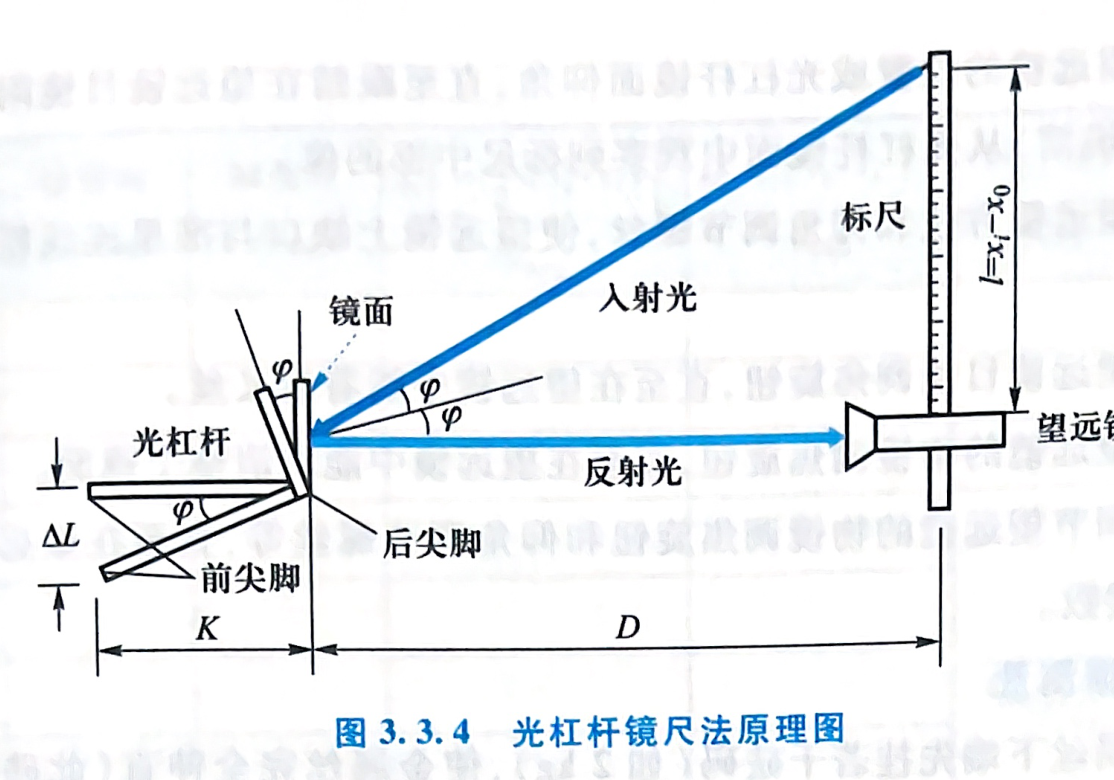
\includegraphics[width=9.3cm]{figures/young-optical-lever.png}\par
{\small 光杠杆镜尺关系示意图。}\end{center}
\ReportSection{实验内容}
\ReportSubsection{仪器调节}
1. 检查金属丝竖直且未超过弹性限度，施加预载消除松弛。调节光杠杆镜面、望远镜和标尺，使标尺像及十字线清晰。\par
2. 测量金属丝长度、镜尺距离与光杠杆臂长；用螺旋测微计在不同方向测直径五次，记录零点。\par
\ReportSubsection{加卸载测量}
3. 按固定质量步长逐级加载，待标尺像稳定后读取十级位置；再逐级卸载，记录对应的十级位置。\par
4. 对每级加载、卸载读数取均值，计算五组逐差 $l_i$ 和杨氏模量；若两条曲线明显分离，应检查摩擦、松弛或是否超出弹性范围。
\ReportSection{实验仪器}
杨氏模量仪、金属丝、光杠杆、望远镜与标尺、砝码、螺旋测微计、游标卡尺和米尺。直径进入平方项，应重视其测量与零点检查。
\ReportSection{数据记录处理}
逐级载荷下的标尺像位置（cm）：
\begin{center}\small\renewcommand{\arraystretch}{1.35}
\begin{tabular}{|c|c|c|c|}\hline
级数 & 加载 & 卸载 & 均值\\\hline
0 & \Field[10mm]{load_up_01} & \Field[10mm]{load_down_01} & \Field[10mm]{load_mean_01}\\\hline
1 & \Field[10mm]{load_up_02} & \Field[10mm]{load_down_02} & \Field[10mm]{load_mean_02}\\\hline
2 & \Field[10mm]{load_up_03} & \Field[10mm]{load_down_03} & \Field[10mm]{load_mean_03}\\\hline
3 & \Field[10mm]{load_up_04} & \Field[10mm]{load_down_04} & \Field[10mm]{load_mean_04}\\\hline
4 & \Field[10mm]{load_up_05} & \Field[10mm]{load_down_05} & \Field[10mm]{load_mean_05}\\\hline
5 & \Field[10mm]{load_up_06} & \Field[10mm]{load_down_06} & \Field[10mm]{load_mean_06}\\\hline
6 & \Field[10mm]{load_up_07} & \Field[10mm]{load_down_07} & \Field[10mm]{load_mean_07}\\\hline
7 & \Field[10mm]{load_up_08} & \Field[10mm]{load_down_08} & \Field[10mm]{load_mean_08}\\\hline
8 & \Field[10mm]{load_up_09} & \Field[10mm]{load_down_09} & \Field[10mm]{load_mean_09}\\\hline
9 & \Field[10mm]{load_up_10} & \Field[10mm]{load_down_10} & \Field[10mm]{load_mean_10}\\\hline
\end{tabular}
\end{center}
\noindent 每级质量增量 $\delta m=\Field{mass_step_kg}$ kg；预载质量 $\Field{preload_kg}$ kg。
\par\noindent 金属丝直径（mm）：
\begin{center}\small\renewcommand{\arraystretch}{1.35}
\begin{tabular}{|c|c|}\hline
序号 & 直径\\\hline
1 & \Field[10mm]{diameter_01}\\\hline
2 & \Field[10mm]{diameter_02}\\\hline
3 & \Field[10mm]{diameter_03}\\\hline
4 & \Field[10mm]{diameter_04}\\\hline
5 & \Field[10mm]{diameter_05}\\\hline
\end{tabular}
\end{center}
\ReportSection{数据记录处理（续）}
\noindent $L=\Field{wire_length_cm}$ cm，$D=\Field{mirror_distance_cm}$ cm，
$K=\Field{lever_arm_cm}$ cm；当地 $g=\Field{gravity_ms2}$ m/s$^2$。
\par\noindent 逐差 $l_i=|x_{i+5}-x_i|$（cm）：
\begin{center}\small\renewcommand{\arraystretch}{1.35}
\begin{tabular}{|c|c|}\hline
$i$ & $l_i$\\\hline
1 & \Field[10mm]{load_difference_00}\\\hline
2 & \Field[10mm]{load_difference_01}\\\hline
3 & \Field[10mm]{load_difference_02}\\\hline
4 & \Field[10mm]{load_difference_03}\\\hline
5 & \Field[10mm]{load_difference_04}\\\hline
\end{tabular}
\end{center}
\[\bar d=(\MathField{diameter_mean_mm}\pm\MathField{diameter_mean_u_mm})\,\mathrm{mm},\quad
\bar l=(\MathField{difference_mean_cm}\pm\MathField{difference_mean_u_cm})\,\mathrm{cm},\quad
E=(\MathField{young_modulus_pa}\pm\MathField{young_uncertainty_pa})\,\mathrm{Pa}.\]
\noindent 与参考值 $\MathField{reference_modulus_pa}$ Pa 的百分差为 $\Field{young_error_percent}\%$。

\ReportSection{加载与卸载曲线}
以加载质量为横轴、望远镜标尺像位置为纵轴，绘出加载、卸载和两者均值。图形用于检查数据是否近似线性及是否存在明显滞后；点均由本次十级读数生成。
\begin{center}\begin{tikzpicture}
\begin{axis}[width=.88\textwidth,height=7cm,xlabel={加载质量/kg},ylabel={标尺像位置/cm},grid=both,legend pos=north west]
\addplot+[mark=*,blue] coordinates {\PlotCoordinates{young_load_up_points}};\addlegendentry{加载}
\addplot+[mark=square*,orange] coordinates {\PlotCoordinates{young_load_down_points}};\addlegendentry{卸载}
\addplot+[mark=triangle*,black] coordinates {\PlotCoordinates{young_load_mean_points}};\addlegendentry{均值}
\end{axis}\end{tikzpicture}\end{center}
\ReportSection{讨论与分析}
\ReportSubsection{加载与卸载}
图中的加载、卸载及均值曲线用于检查弹性区的近似线性。若加载与卸载差距大，可能有机械滞后、支架松动或读数尚未稳定，不能仅凭平均值掩盖异常。\par
\ReportSubsection{不确定度}
金属丝直径以平方进入公式，直径偏差会被放大；镜尺距离和臂长误差以及望远镜视差也应检查。逐差法利用较大的位移可减弱标尺像单次读数的相对误差，但不能消除系统误差。\par
\ReportSubsection{思考题}
为何先施加预载？使钢丝和装置进入稳定受力状态。为何沿多个方向测直径？金属丝可能略呈椭圆，多方位测量有助于估计截面尺寸。
\ReportSection{实验结论}
通过光杠杆和五级逐差法得到 $E=(\MathField{young_modulus_pa}\pm\MathField{young_uncertainty_pa})\,\mathrm{Pa}$，与输入参考值的百分差为 $\Field{young_error_percent}\%$。应结合加载卸载一致性与直径测量评价结果。

\ReportRecord
% ===== 原始数据图片插入区 =====
\end{document}
